\chapter{Experiments}
\label{cha:experiments}

\Autosectionref{sec:experimental-setup} of the \nameref{cha:experiments} chapter will describe the methodology and rationale behind the two experiments conducted in this thesis. The first experiment, presented in \autoref{subsec:benchmarking-setup}, assesses GeoGPT's ability to solve common \acrshort{acr:gis} tasks through a new \acrshort{acr:gis} benchmarking dataset. The other experiment, presented in \autoref{subsec:prompt-quality-test-setup}, will assess the importance of the quality of the prompt passed from the user to GeoGPT. \Autosectionref{sec:datasets} lists the datasets used in the experiments. \Autosectionref{sec:experimental-results} presents the experimental results and offers interpretations of the findings from the experiments. It will also present several example results, including screenshots of the application and code that generated by GeoGPT.

\section{Experimental Setup}
\label{sec:experimental-setup}

\begin{comment}
Trying and failing is a major part of research. However, to have a chance of success you need a plan driving the experimental research, just as you need a plan for your literature search. Further, plans are made to be revised and this revision ensures that any further decisions made are in line with the work already completed.

The plan should include what experiments or series of experiments are planned and what questions the individual or set of experiments aim to answer. Such questions should be connected to your research questions, so that in the evaluation of your results you can discuss the results wrt to the research questions.
\end{comment}

\begin{comment}
The experimental setup should include all data --- parameters, etc. --- that would allow a person to repeat your experiments.
This will thus be the actual instantiation for each experiment of the general architecture described in Chapter~\ref{cha:architecture}.
\end{comment}

% The experiments conducted using the above-mentioned \acrshort{acr:gis} benchmark are divided into two approaches. The first approach, presented in \autoref{subsec:benchmarking-setup}, is intended to evaluate GeoGPT's ability to solve a variety of geospatial tasks. The second approach, presented in \autoref{subsec:prompt-quality-test-setup}, aims to uncover the importance of the quality of the initial user prompt. \Autosubsectionref{subsec:hardware-and-model-version} describes the hardware on which the experiments were executed, and the specific \acrshortpl{acr:llm} that were used.

This section will explain the concept and setup of the two experiments mentioned in the paragraph above. \Autosectionref{subsec:benchmarking-setup} will describe the setup for the \acrshort{acr:gis} benchmark experiments, while \autoref{subsec:prompt-quality-test-setup} will explain the setup for the prompt quality experiment. \Autosubsectionref{subsec:hardware-and-model-version} describes the hardware on which the experiments were conducted, and the specific \acrshortpl{acr:llm} that were used.

\subsection[GIS Benchmark Experiment]{\acrshort{acr:gis} Benchmark Experiment}
\label{subsec:benchmarking-setup}

% In order to investigate how an \acrshort{acr:llm}-based \acrshort{acr:gis} agent most comfortably accesses geospatial data, a decision was made to include three different methods for data access in the experiments. The first method for data access is to have the files described in \autoref{sec:datasets} remain untouched. The files would be stored locally on the computer on which the experiments are conducted, and GeoGPT, which runs on the same computer, would be able to interact with the data through the code it generates. These files are made available in GeoGPT's working directory. The second method used is to load the data into a spatial \acrshort{acr:sql} database and provide the model with database schemas that can be used to generate queries. The datasets were uploaded to a Dockerized PostGIS database using QGIS's DB Manager plugin. The third method for data access is to use the \acrshort{acr:ogc} \acrshort{acr:api} Features standard. This method exposes the data stored in the PostGIS database through a web \acrshort{acr:api} that allows consumers of the \acrshort{acr:api} to download the data over \acrshort{acr:http} as GeoJSON.

The first experiment will measure the abilities of GeoGPT three agent types to produce correct answers. It will also measure cost and time taken to generate answers, and the agent's ability to produce similar answers consistently (repeatability). To do this, a benchmarking dataset was constructed. This is a set of 12 GIS-related questions with corresponding correct answers, and can be viewed in its entirety in \autoref{tbl:questions-quantitative}. The \acrshort{acr:gis} benchmark experiment will seek to compare the performance of GeoGPT's three agents. Each of the 12 questions will be asked three times per agent type. Thus, the total number of test runs becomes the following:

$$12 \text{ questions} \cdot 3 \text{ agent types} \cdot 3 \text{ repetitions} = 108 \text{ tests}$$

The following sections, named \enquote{\nameref{subsubsec:outcome-evaluation}}, \enquote{\nameref{subsubsec:cost-and-duration}}, \enquote{\nameref{subsubsec:repeatability}}, will go into detail on the different ways that the results are evaluated.

\subsubsection{Outcome Evaluation}
\label{subsubsec:outcome-evaluation}

Each of the 108 GeoGPT-generated answers will be manually evaluated based on how well the question was answered, and this outcome will be annotated as one of the following: \textit{success}, \textit{partial success}, and \textit{failure}. \autoref{tbl:test-outcome-enum} shows the guidelines used when assigning outcome scores.

\begin{table}[htbp]
    \centering
    \caption[Guidelines for evaluating outcome of tests]{Guidelines for evaluating outcome of tests}
    \label{tbl:test-outcome-enum}
    \begin{tabularx}{0.9\textwidth}{p{3cm}X}
        \toprule
        \textbf{Outcome} & \textbf{Guideline}                                                                                                                                                                                  \\
        \midrule
        Success          & The question was answered correctly and little to no follow-up from the user was required to produce the desired outcome. No false assumptions were made by the system when answering the question. \\
        Partial Success  & Portions of the question were answered correctly or semi-correctly, and/or some follow-up from the user was required to guide the system toward the solution.                                       \\
        Failure          & The question was answered incorrectly, and/or false assumptions were made by the system while attempting to answer the question.                                                                    \\
        \bottomrule
    \end{tabularx}
\end{table}


\subsubsection{Cost and Duration}
\label{subsubsec:cost-and-duration}

The application is hooked up to LangChain AI's tracing system, \textit{LangSmith}.\footnote{\url{https://www.langchain.com/langsmith} (last visited on 2nd June 2024)} Apart from being a useful tool for debugging purposes, it provides a simple way to obtain detailed data on token and time usage for a particular run, as well as the total cost of the run, in American dollars. Further details, and screenshots of LangSmith's interface, can be found in \autoref{app:langsmith}.

Box plots will be used to compare these three metrics for the different agents. The box plots follow the description for box plots found on Wikipedia.\footnote{\url{https://matplotlib.org/stable/api/_as_gen/matplotlib.pyplot.boxplot.html} (last visited on 2nd June 2024)}\footnote{\url{https://en.wikipedia.org/wiki/Box_plot} (last visited on 2nd June 2024)} Box plots allow us to easily see where the 0th ($Q_0$), 25th ($Q_1$), 50th ($Q_2$), 75th ($Q_3$), and 100th ($Q_4$) percentiles of the datasets lie, as well as the dataset's outliers. Outliers are those data points that fall more than 50\% outside the interquartile range, which is the distance between $Q_3$ and $Q_1$ in each direction.

\subsubsection{Repeatability}
\label{subsubsec:repeatability}

Another aspect that the \acrshort{acr:gis} benchmark experiment will try to evaluate, is the consistency of the system --- its ability to produce similar responses, repeatedly. The outcomes scores are encoded using the ordinal encoding presented \autoref{tbl:outcome-encoding}. A higher value indicates a better outcome. Standard deviations are calculated for each triplet of identical test samples (samples where the question and the agent type remained the same), using these encoded outcomes. This will serve as a suitable measure for assessing repeatability.

\begin{table}[htbp]
    \centering
    \caption{Ordinal encodings for outcome scores}
    \label{tbl:outcome-encoding}
    \begin{tabularx}{0.5\textwidth}{XX}
        \toprule
        \textbf{Outcome} & \textbf{Encoded Value} \\
        \midrule
        Success          & 2                      \\
        Partial Success  & 1                      \\
        Failure          & 0                      \\
        \bottomrule
    \end{tabularx}
\end{table}


\subsection{Prompt Quality Experiment}
\label{subsec:prompt-quality-test-setup}

A second experiment is constructed to evaluate the importance of the initial question/prompt from the user. As stated in the \nameref{sec:background-and-motivation} chapter, part of the motivation for developing an \acrshort{acr:llm}-based \acrshort{acr:gis} like GeoGPT is to make \acrshort{acr:gis} more accessible to non-experts. It is therefore interesting to assess the extent to which a carefully constructed prompt by a \acrshort{acr:gis} expert can enhance the system's output.

For these experiments, the three hardest questions from the \acrshort{acr:gis} benchmark experiment were picked. Then, for each of these three questions, a \textit{novice}-level and an \textit{expert}-level prompt was constructed. The novice-level prompt is as simple as possible, while the expert-level prompt is more elaborate and written as a step-by-step recipe for solving the problem. Despite their differences, the prompts should ideally produce the same answer.

\subsection[Hardware and LLM Version]{Hardware and \acrshort{acr:llm} Version}
\label{subsec:hardware-and-model-version}

All experiments were conducted on a Lenovo ThinkPad E490, which has an Intel{\textregistered} Core\texttrademark{} i7-8565U CPU @ 1.80GHz processor, 15.8 GB usable \acrshort{acr:ram}, and 256 GB \acrshort{acr:ssd} storage. Everything but the \acrshort{acr:llm} inference was done locally. \acrshort{acr:llm} inference (text generation) was done using OpenAI's Inference \acrshort{acr:api}.

It is worth noting that two slightly different models were used during testing. This is due the release of the \texttt{gpt-4-turbo-2024-04-09} model in mid-April. According to OpenAI, \enquote{this new model is better at math, logical reasoning, and coding} compared to \texttt{gpt-4-0125-preview},\footnote{OpenAI has a GitHub repository containing the code they use to evaluate their \glspl{acr:llm} and benchmark results for OpenAI models and reference models from other companies: \url{https://github.com/openai/simple-evals} (last visited on 2nd June 2024)} which is the model that was used for the first test runs. At \texttt{gpt-4-turbo-2024-04-09}'s release, a decision was made to use this for the remaining experiments. The experiments that had already been conducted were not re-run due to time constraints and a confidence that these slight model upgrades would not significantly change the outcome of the experiments.


\section{Datasets}
\label{sec:datasets}

A total of eighteen datasets were used in the experiments, all downloaded from a website called \enquote{Geofabrik}.\footnote{\url{https://download.geofabrik.de/europe/norway.html} (last visited on 2nd June 2024)} \textit{Geofabrik}, which is German for \enquote{geo factory}, is a company that \enquote{extract, select, and process free geodata}. They have gathered data from OpenStreetMap and published them as a collection of shapefiles, dividing them into categories such as \enquote{places of worship}, \enquote{points of interest}, and \enquote{traffic}. Data can be downloaded for different regions of the world, but for the experiments conducted in this thesis, only data for Norway was used. \autoref{tbl:datasets} lists the datasets, along with short descriptions of their contents, and the number of features for each dataset. Common for all datasets is their \emph{fclass} attribute, which is short for \emph{feature class}. Some datasets have additional attributes, such as the \emph{maxspeed} attribute in the road dataset and the \emph{type} attribute in the building dataset. \autoref{fig:datasets-trondheim} shows a plot containing four selected datasets, constrained to a bounding box of Trondheim. This plot was created by GeoGPT.

\begin{longtable}{p{3cm}p{2cm}p{5.7cm}p{2.5cm}}
    \caption{Datasets used in the experiments}                                                                                                                                                                                                              \\
    \label{tbl:datasets}                                                                                                                                                                                                                                    \\
    \toprule
    \textbf{Dataset}   & \textbf{Type} & \textbf{Description}                                                                                                                                                                         & \textbf{\#Features} \\
    \midrule
    \endfirsthead

    \multicolumn{4}{c}{{\bfseries Table \thetable\ continued from previous page}}                                                                                                                                                                           \\
    \toprule
    \textbf{Dataset}   & \textbf{Type} & \textbf{Description}                                                                                                                                                                         & \textbf{\#Features} \\
    \midrule
    \endhead

    \midrule
    \multicolumn{4}{r}{Continued on next page}                                                                                                                                                                                                              \\
    \midrule
    \endfoot

    \bottomrule
    \endlastfoot

    Buildings          & Polygon       & Contains building outlines. Its \emph{type} attribute can have values like \enquote{house}, \enquote{university}, and \enquote{restaurant}.                                                  & 4,147,645           \\
    Land Use           & Polygon       & Represents areas designated to different purposes and activities. Its \emph{fclass} attribute can have values like \enquote{forest}, \enquote{farmland}, and \enquote{residential}.          & 541,452             \\
    Natural            & Point         & Contains outlines of various objects found in nature. Its \emph{fclass} attribute can have values like \enquote{beach}, \enquote{glacier}, and \enquote{cave\_entrance}.                     & 119,725             \\
    Natural            & Polygon       & Similar to the point data equivalent.                                                                                                                                                        & 6,665               \\
    Places of Worship  & Point         & Common values for \emph{fclass} attribute: \enquote{christian}, \enquote{buddhist}, and \enquote{muslim}.                                                                                    & 311                 \\
    Places of Worship  & Polygon       & Similar to the point data equivalent.                                                                                                                                                        & 2,520               \\
    Places             & Point         & Common values for \emph{fclass} attribute: \enquote{farm}, \enquote{village}, and \enquote{island}.                                                                                          & 178,997             \\
    Places             & Polygon       & Similar to the point data equivalent.                                                                                                                                                        & 5,689               \\
    Points of Interest & Point         & Common values for \emph{fclass} attribute: \enquote{tourist\_info}, \enquote{bench}, and \enquote{kindergarten}.                                                                             & 117,677             \\
    Points of Interest & Polygon       & Similar to the point data equivalent.                                                                                                                                                        & 45,825              \\
    Railways           & Line          & Common values for \emph{fclass} attribute: \enquote{rail}, \enquote{subway}, and \enquote{tram}. Also has True/False attributes \emph{bridge} and \emph{tunnel}.                             & 14,008              \\
    Roads              & Line          & Common values for \emph{fclass} attribute: \enquote{rail}, \enquote{subway}, and \enquote{tram}. Has additional attributes \emph{oneway}, \emph{maxspeed}, \emph{bridge}, and \emph{tunnel}. & 1,741,929           \\
    Traffic            & Point         & Common values for \emph{fclass} attribute: \enquote{crossing}, \enquote{street\_lamp}, and \enquote{parking}.                                                                                & 98,860              \\
    Traffic            & Polygon       & Common values for \emph{fclass} attribute: \enquote{parking}, \enquote{pier}, and \enquote{dam}.                                                                                             & 45,623              \\
    Transport          & Point         & Common values for \emph{fclass} attribute: \enquote{bus\_stop}, \enquote{ferry\_terminal}, and \enquote{railway\_station}.                                                                   & 91,627              \\
    Transport          & Polygon       & Similar to the point data equivalent.                                                                                                                                                        & 935                 \\
    Water              & Polygon       & Common values for \emph{fclass} attribute: \enquote{water}, \enquote{wetland}, and \enquote{river\_bank}.                                                                                    & 1,861,199           \\
    Waterways          & Line          & Common values for \emph{fclass} attribute: \enquote{stream}, \enquote{river}, and \enquote{canal}.                                                                                           & 833,253             \\
\end{longtable}


\begin{figure}
    \centering
    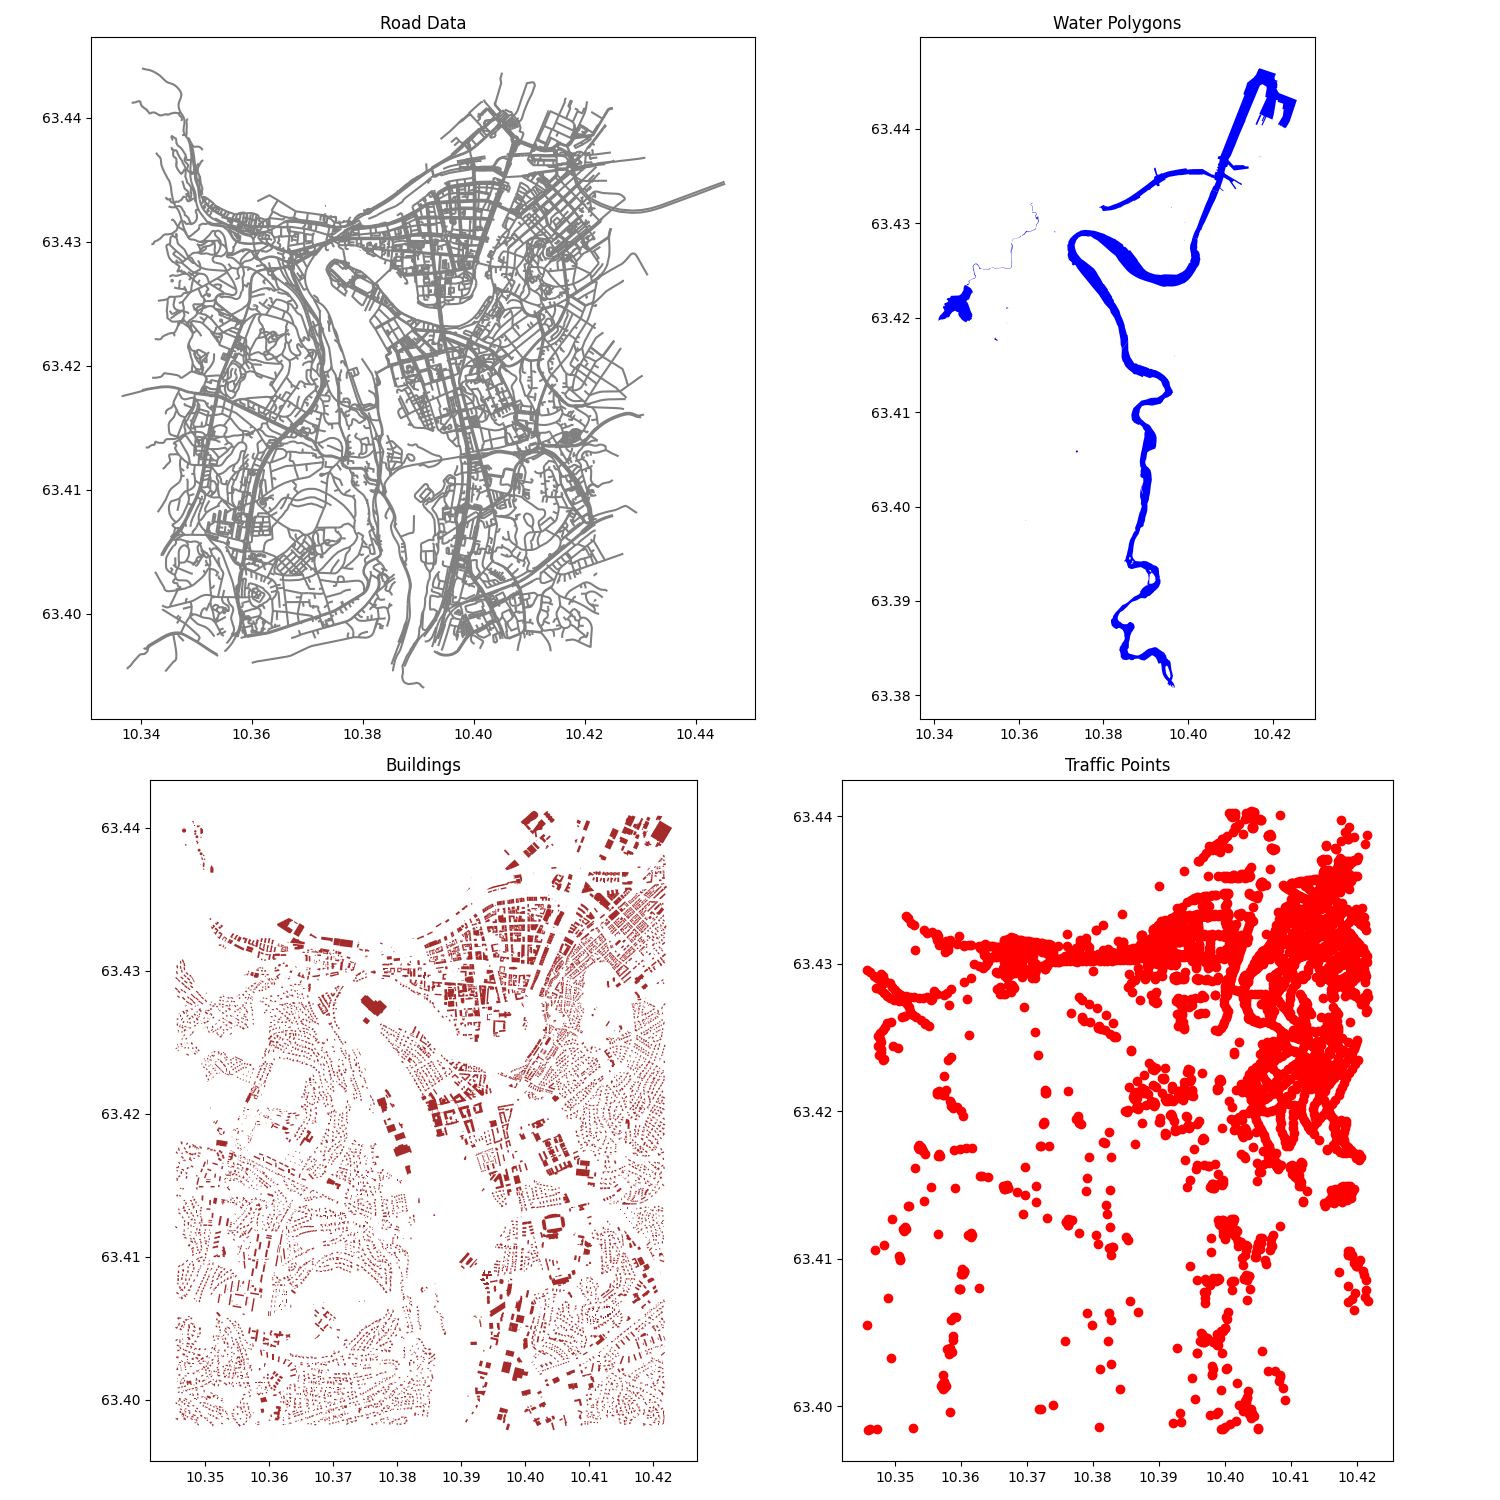
\includegraphics[width=\textwidth]{trondheim_datasets.png}
    \caption[A plot of four selected datasets constrained to a polygon of Trondheim]{A plot of four selected datasets constrained to a polygon of Trondheim. From top-left, clockwise: road lines, water polygons, traffic points, and building polygons. These plots were generated by GeoGPT.}
    \label{fig:datasets-trondheim}
\end{figure}

\FloatBarrier


\section{Experimental Results}
\label{sec:experimental-results}

\begin{comment}
Results should be clearly displayed and should provide a suitable representation of your results for the points you wish to make.
Graphs should be labelled in a legible font. If more than one result is displayed in the same graph, then these should be clearly marked.
Please choose carefully rather than presenting every result. Too much information is hard to read and often hides the key information you wish to present. Make use of statistical methods when presenting results, where possible to strengthen the results.
Further, the format of the presentation of results should be chosen based on what issues in the results you wish to highlight.
You may wish to present a subset in the experimental section and provide additional results in an appendix.
Point out specifics here but save the overall/general discussion to the Discussion chapter.
\end{comment}

\Autosubsectionref{subsec:quantitative-results} and \autoref{subsec:prompt-quality-test-results} will present the outcome of the experiments presented in \autoref{subsec:benchmarking-setup} and \autoref{subsec:prompt-quality-test-setup}, respectively. Visualizations for this section were created using Matplotlib,\footnote{\url{https://matplotlib.org/} (last visited on 2nd June 2024)} a Python library suitable for creating bar charts, box plots, etc.


\subsection[GIS Benchmark Experiment --- Results]{\acrshort{acr:gis} Benchmark --- Results}
\label{subsec:quantitative-results}

\subsubsection{Outcome Evaluation}

\autoref{fig:outcome-distribution} shows a bar charts for the outcome distribution between GeoGPT's three agents. The \acrshort{acr:ogc} \acrshort{acr:api} Features agent and the Python agent have comparable results, whereas the \acrshort{acr:sql} agent performs significantly better than the other two. The \acrshort{acr:sql} agent has a success rate of 69.4\%, while the other two share a success rate of 38.9\%. Possible reasons for this are discussed in \autoref{sec:why-sql-better} of the \nameref{cha:discussion}.

\begin{figure}[htbp]
    \centering
    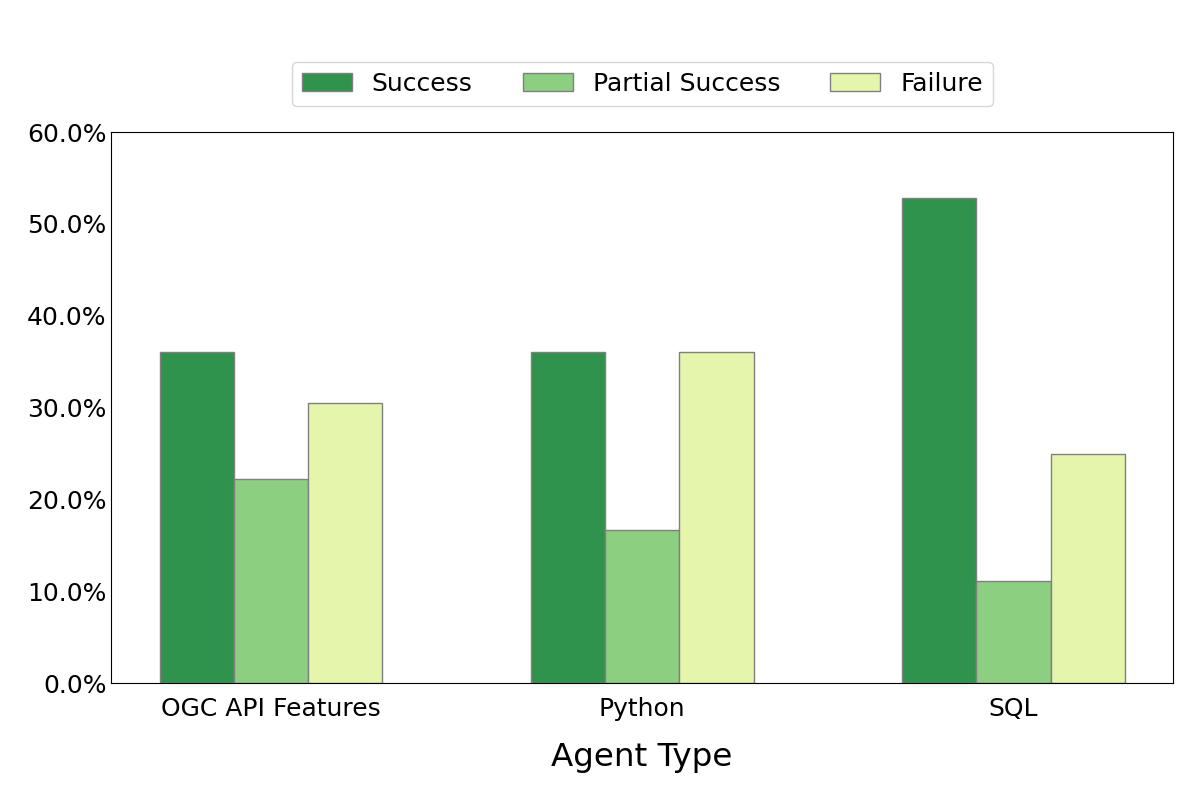
\includegraphics[width=\textwidth]{outcome_distribution_bar_chart.png}
    \caption[Outcome distribution between GeoGPT's different agent types]{Outcome distribution between GeoGPT's different agent types. The \acrshort{acr:ogc} \acrshort{acr:api} Features and Python agents perform similarly, while the \acrshort{acr:sql} agent outperforms them by a significant margin.}
    \label{fig:outcome-distribution}
\end{figure}

\subsubsection{Cost and Duration}

\autoref{fig:duration-box-plot} displays a box plot with a logarithmic y-axis that shows task durations between the different agent types. Here we can see that the \acrshort{acr:sql} agent spends the least amount of time per task. The \acrshort{acr:ogc} \acrshort{acr:api} Features agent has a slightly higher median, but with a few time-consuming outliers. The Python agent is the odd one out with a median of $\sim 82$ seconds, a $Q3 \sim 293$ seconds, and a $Q4 \sim 984$ seconds. The large gap from the Python agent to the other two agents it largely due to the Python agent's tendency to load large datasets into memory. For instance, when attempting the task of calculating the difference between the polygon outlining Oslo and water polygons (see \autoref{tbl:questions-quantitative} for the task formulation), the Python agent used nearly 40 minutes on the entire task. $94\%$ of the time was spent executing the code in \autoref{code:python-oslo-water-diff}. The main reason for the long execution time is line 8, where the whole \texttt{osm\_landuse\_polygons.shp} dataset is loaded into memory. This dataset has a size of $\sim 1.4 \text{ GB}$ and a total of 1,861,199 polygon features, and loading such amounts of data in this way is very time-consuming. The Python agent was the only agent with such issues because the \acrshort{acr:ogc} \acrshort{acr:api} Features agent is limited to 10,000 features per request, and the \acrshort{acr:sql} agent does not load the data into memory like the other agents do.

\begin{figure}[htbp]
    \centering
    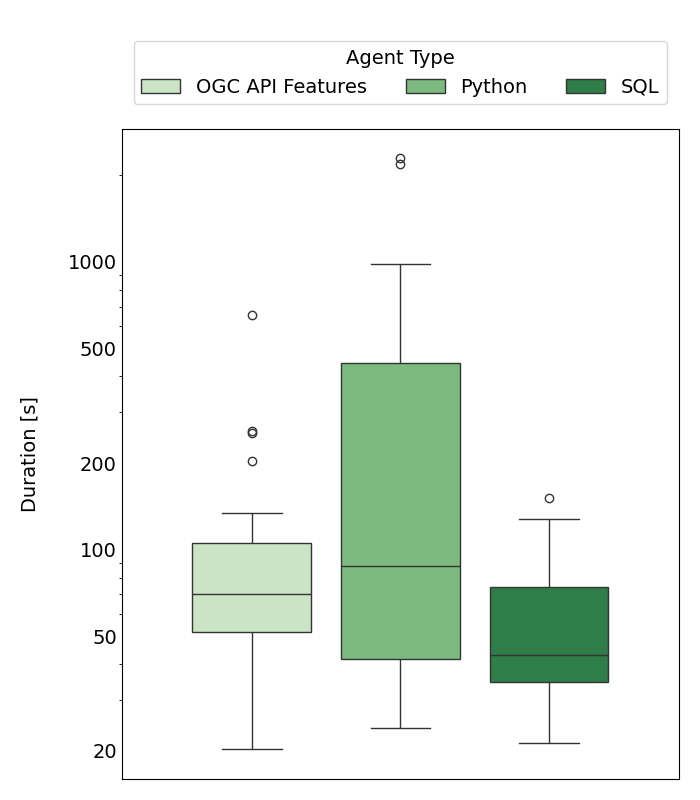
\includegraphics[width=0.6\textwidth]{duration_box_plot.png}
    \caption[Box plots comparing the time taken to generate answers between GeoGPT's agent types]{Box plots comparing the time taken to generate answers between GeoGPT's agent types. Again, the \acrshort{acr:sql} agent performs best, while the Python agent is the odd one out with very slow times compared to the other two.}
    \label{fig:duration-box-plot}
\end{figure}

\FloatBarrier

\begin{lstlisting}[
    language=Python,
    caption={[GeoGPT-generated Python code aimed at computing the difference between the outline of Oslo and residental features within it]GeoGPT-generated Python code aimed at computing the difference between the outline of Oslo, the Norwegian capital, and residental features within it. The execution time of this code block was $\sim 36$ minutes, mostly due to line 8.},
    label=code:python-oslo-water-diff,
    float
]
    import geopandas as gpd

    # Paths to the shapefiles
    landuse_path = '/tmp/tmpsutdy6it/osm_landuse_polygons.shp'
    places_path = '/tmp/tmpsutdy6it/osm_places_polygons.shp'
    
    # Load the data from shapefiles
    landuse_gdf = gpd.read_file(landuse_path)
    places_gdf = gpd.read_file(places_path)
    
    # Filter out 'residential' areas from the landuse data
    residential_gdf = landuse_gdf[landuse_gdf['fclass'] == 'residential']
     
    # Compute the spatial difference to exclude residential areas from the places data
    oslo_outline = gpd.overlay(places_gdf, residential_gdf, how='difference')
    
    # Path for the output GeoJSON file
    output_path = '/tmp/tmpsutdy6it/oslo_outline_no_residential.geojson'
    
    # Save the resulting GeoDataFrame to a GeoJSON file
    oslo_outline.to_file(output_path, driver='GeoJSON')
    
    # Output the path to the saved file
    print(output_path)    
\end{lstlisting}

\autoref{fig:cost-and-tokens} shows box plots for token usage and cost per run. Naturally, these figures appear very similar, since prices for the input tokens and generated output tokens are fixed for the models used. According to OpenAI's webpages,\footnote{\url{https://openai.com/pricing} (last visited 2nd June 2024)} they charge $\$10$ per million input tokens and $\$30$ per million output tokens for their \acrshort{acr:gpt}-4 Turbo model. From the results of the experiments, a ratio of approximately $\text{\$}10.7$ per million tokens --- either input \textit{or} output --- was calculated, which is closest to the input token price. This shows that \textit{a lot} more input tokens were used, compared to output tokens.

\begin{figure}[htbp]
    \centering
    \begin{subfigure}[b]{0.48\textwidth}
        \centering
        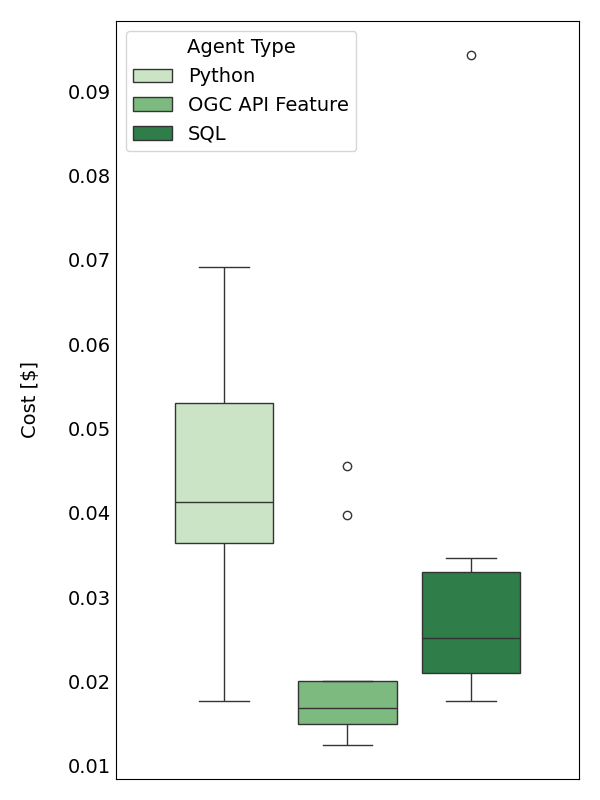
\includegraphics[width=\textwidth]{cost_box_plot.png}
        \caption{Average cost per answer between the agent types}
        \label{fig:cost-box-plot}
    \end{subfigure}
    \hfill
    \begin{subfigure}[b]{0.48\textwidth}
        \centering
        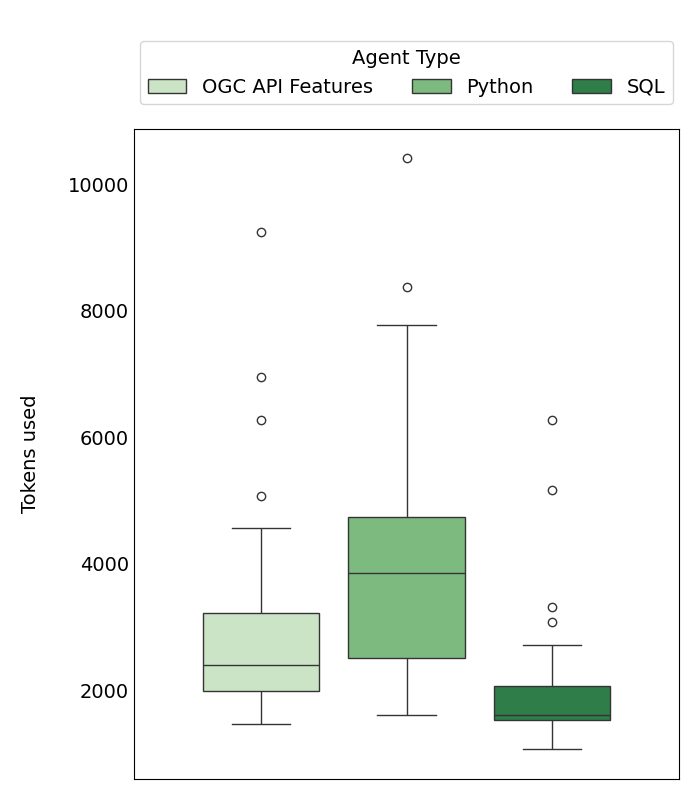
\includegraphics[width=\textwidth]{tokens_box_plot.png}
        \caption{Average token usage per answer between the agent types}
        \label{fig:tokens-box-plot}
    \end{subfigure}
    \caption[Cost and token usage between GeoGPT's different agent types]{Cost and token usage between GeoGPT's different agent types. These plots are highly correlated, but will differ somewhat because of the ratio between input and output tokens.}
    \label{fig:cost-and-tokens}
\end{figure}

An observation that can be made from the correlation matrices in \autoref{fig:correlation-matrices} is that the correlation between duration and token usage is inconsistent between the agent types. The \acrshort{acr:ogc} \acrshort{acr:api} Features agent and \acrshort{acr:sql} agent have strong correlation between these metrics, but the Python agent has next to none. This supports the observation that, for the Python agent, code execution time, particularly the time spent on expensive imports, is likely the main contributor towards the total run time.

Another observation that can be made from the \autoref{fig:correlation-matrices} is the slight negative correlation between the encoded outcome and each of the following variables: token usage, duration, and total cost. This suggests that a task that takes longer to complete, and has a higher token usage, is \textit{less} likely to produce a successful outcome. Possible reasons as to why this is the case will be explored in \autoref{subsec:dead-ends} in the \nameref{cha:discussion}.

\begin{figure}[htp]
    \centering

    \begin{subfigure}[b]{\textwidth}
        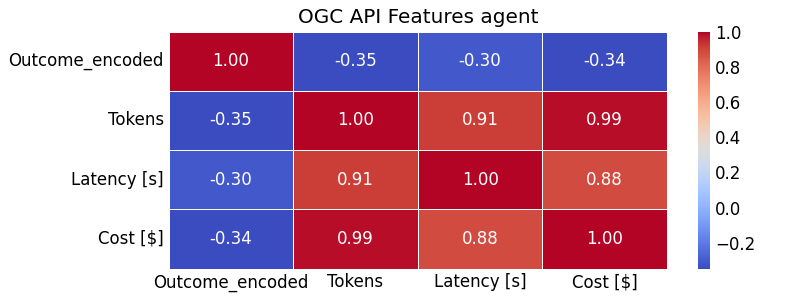
\includegraphics[width=\textwidth]{correlation_matrix_oaf.png}
        \caption{Correlation matrix for the \acrshort{acr:ogc} \acrshort{acr:api} Features agent}
        \label{fig:sub1}
    \end{subfigure}

    \vspace{1cm}

    \begin{subfigure}[b]{\textwidth}
        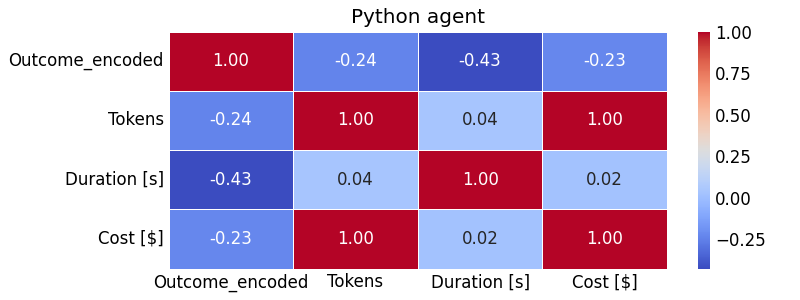
\includegraphics[width=\textwidth]{correlation_matrix_python.png}
        \caption{Correlation matrix for the Python agent}
        \label{fig:sub2}
    \end{subfigure}

    \vspace{1cm}

    \begin{subfigure}[b]{\textwidth}
        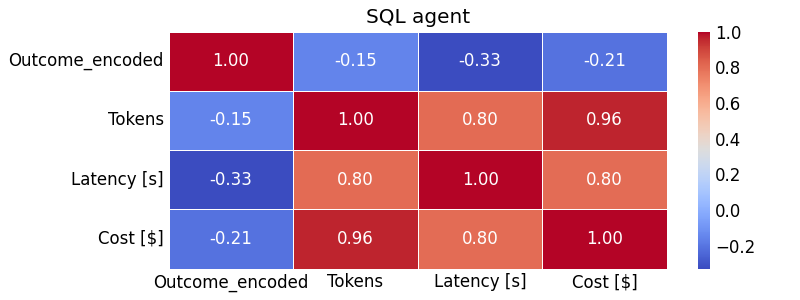
\includegraphics[width=\textwidth]{correlation_matrix_sql.png}
        \caption{Correlation matrix for the \acrshort{acr:sql} agent}
        \label{fig:sub3}
    \end{subfigure}

    \caption{Correlation matrices for the metrics recorded during the \acrshort{acr:gis} benchmark experiment for the three agent types}
    \label{fig:correlation-matrices}
\end{figure}

\subsubsection{Repeatability}

\autoref{tbl:stddev-by-agent-type} shows the average standard deviation of the outcomes for each agent type, as well as the mean of these three standard deviations. These numbers indicate that there is a notable amount of inconsistency in GeoGPT's answers when task and agent type stays the same, on average deviating with more than a third of an outcome category (0.376 for the encoded values).

\begin{table}[htbp]
    \centering
    \caption{Standard deviations of encoded outcomes for GeoGPT's agent types}
    \label{tbl:stddev-by-agent-type}
    \begin{tabularx}{0.7\textwidth}{XX}
        \toprule
        \textbf{Agent Type}                            & \textbf{Outcome Std. Deviation} \\
        \midrule
        \acrshort{acr:ogc} \acrshort{acr:api} Features & 0.552                           \\
        Python                                         & 0.337                           \\
        \acrshort{acr:sql}                             & 0.241                           \\
        \midrule
        \textbf{Mean}                                  & 0.376                           \\
        \bottomrule
    \end{tabularx}
\end{table}

\FloatBarrier

\subsubsection{Successful Responses}

% 6df94421-6c7c-470a-af8e-7013f3bc547f
\autoref{fig:glomma-counties-sql-successful} shows a successful response from GeoGPT's \acrshort{acr:sql} agent when asked how many counties the Glomma river runs through.\footnote{This run was not part of the results used for evaluation due to a bug in the \texttt{sql\_db\_query} tool that caused it to unnecessarily execute queries twice. GeoGPT's response would not be different had the bug not been present for the run, but it would have taken longer to complete.} GeoGPT correctly lists all four correct counties in a numbered list. \autoref{code:glomma-counties-sql} shows the code generated by GeoGPT for the second invocation of \texttt{sql\_db\_query}. The second invocation is nearly identical to the first one, but in the first invocation the geometry column was not included in the response, meaning GeoGPT was unable to add the results to the map. The tool informs GeoGPT about this, and the agent therefore decided to run the query again, now making sure to include the geometry column in the query result, before adding the resulting GeoJSON file to the map using the \texttt{add\_geojson\_to\_map} tool. A follow-up message instructed GeoGPT to \enquote{Add Glomma to the map}, allowing for visual verification that the answer it gave was correct.

\begin{figure}[htbp]
    \centering
    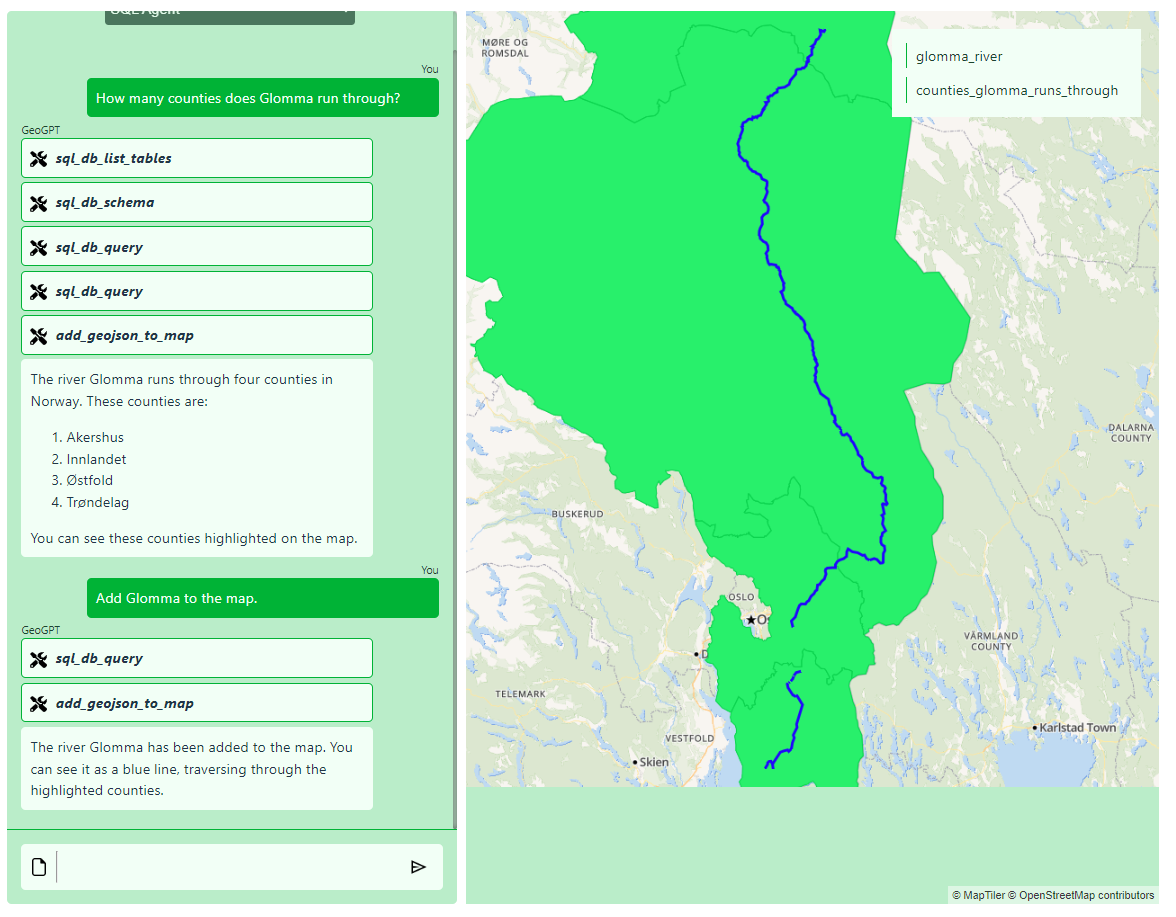
\includegraphics[width=\textwidth]{glomma_counties_sql_22.png}
    \caption[Successful response from GeoGPT's SQL agent when asked how many counties the Glomma river runs through]{Successful response from GeoGPT's \acrshort{acr:sql} agent when asked how many counties the Glomma river runs through. Using the tools available to it, GeoGPT's \acrshort{acr:sql} agent was able to to find that the river Glomma runs through the following counties: Akershus, Innlandet, Østfold, and Trøndelag. A follow-up message was added to make GeoGPT add the river geometries to the map, for verification of its results.}
    \label{fig:glomma-counties-sql-successful}
\end{figure}

\FloatBarrier

\begin{lstlisting}[
    language=sql,
    caption={[GeoGPT-generated SQL code to retrieve the counties that the Glomma river runs through]GeoGPT-generated \acrshort{acr:sql} code to retrieve the counties that the Glomma river runs through. The \texttt{ST\_Intersects} function from PostGIS was used to find the intersection between the river data and the county polygons, and the names and geometries of the counties was included in the result.},
    label=code:glomma-counties-sql,
]
WITH river AS (
    SELECT geom 
    FROM osm_waterways_lines 
    WHERE fclass = 'river' AND name ILIKE 'Glomma'
),

places AS (
    SELECT geom, name 
    FROM osm_places_polygons 
    WHERE fclass = 'county'
)

SELECT DISTINCT places.name AS county_name, places.geom AS geom
FROM river, places
WHERE ST_Intersects(river.geom, places.geom);    
\end{lstlisting}

\FloatBarrier

\autoref{fig:trees-along-munkegata-python-partial-success} shows a partially successful attempt from GeoGPT's Python agent to calculate the number of trees along Munkegata in Trondheim. While setting a definitive answer to such a question is difficult, the correct answer was set to about 100, assuming a 20-meter buffer around the line segments that make up the road. In \autoref{code:python-munkegata-bbox}, we can see how GeoGPT loads the road data around Munkegata in Trondheim, using an approximate bounding box to avoid retrieving roads named \enquote{Munkegata} in other cities. It then filters and saves the loaded data to only include features named Munkegata. In the following code block, shown in \autoref{code:python-trees-count-munkegata}, GeoGPT gets the tree data by filtering the \texttt{osm\_natural\_points} dataset on the \texttt{fclass} attribute, before loading the road data for Munkegata from \autoref{code:python-munkegata-bbox}, converting both datasets to a metric \acrshort{acr:crs}, creating a buffer around the road data, performing an intersection between the buffer, and finally printing the \texttt{tree\_count} to the standard output.

\begin{figure}[htbp]
    \centering
    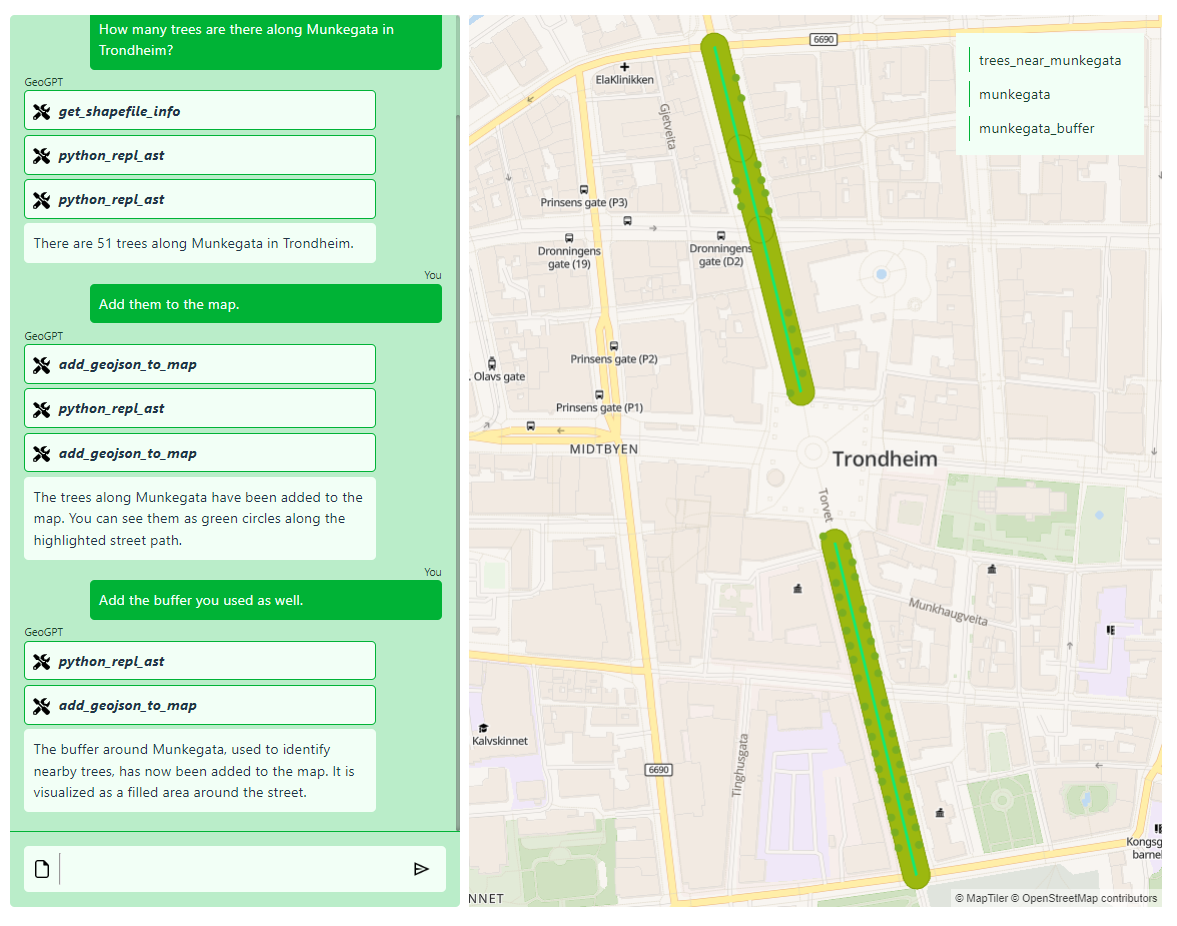
\includegraphics[width=\textwidth]{num_trees_along_munkegata_python_with_buffer.png}
    \caption[Partially successful response from GeoGPT's Python agent when asked how many trees there are along Munkegata in Trondheim]{Partially successful response from GeoGPT's Python agent when asked how many trees there are along Munkegata in Trondheim. It managed to find the road segments corresponding to Munkegata in Trondheim, but created a slightly too small buffer around it, which did not cover all the relevant trees.}
    \label{fig:trees-along-munkegata-python-partial-success}
\end{figure}

\FloatBarrier

\begin{lstlisting}[
    language=python,
    caption={[GeoGPT-generated Python code to retrieve the Munkegata road in Trondheim]GeoGPT-generated Python code to retrieve the Munkegata road in Trondheim. The bounding box, which is generated from \acrshort{acr:gpt}-4's background knowledge, covers a suitable area in the center of Trondheim, where Munkegata is located. This step is important, as a road named \enquote{Munkegata} can also be found in Oslo, which is located in a \textit{completely different} part of Norway.},
    label=code:python-munkegata-bbox,
]
import geopandas as gpd

# Load roads data with a focus on Munkegata
roads_path = '/tmp/tmpl8zsdj6m/osm_roads_lines.shp'
munkegata_bbox = (10.3910, 63.4270, 10.4030, 63.4330) # Approximate bounding box around Munkegata
munkegata_roads = gpd.read_file(roads_path, bbox=munkegata_bbox)

# Filter for Munkegata
munkegata = munkegata_roads[munkegata_roads['name'] == 'Munkegata']

# Save filtered Munkegata road to GeoJSON
munkegata_path = '/tmp/tmpl8zsdj6m/munkegata.geojson'
munkegata.to_file(munkegata_path, driver='GeoJSON')

print(munkegata_path)
\end{lstlisting}

\FloatBarrier

\begin{lstlisting}[
    language=python,
    caption={[GeoGPT-generated Python code to calculate the number of trees along Munkegata in Trondheim]Python code to calculate the number of trees along Munkegata in Trondheim. The datasets were converted to a metric \acrshort{acr:crs} (WGS 84 / UTM zone 33N), before a buffer around the road data from \autoref{code:python-munkegata-bbox} was created and used to find the intersection with the tree data. 51 trees were found, but ideally $\sim 100$ should be returned.},
    label=code:python-trees-count-munkegata,
]
from shapely.geometry import box
import geopandas as gpd

# Load the trees points
natural_points_path = '/tmp/tmpl8zsdj6m/osm_natural_points.shp'
trees = gpd.read_file(natural_points_path)

# Filter for trees
trees = trees[trees['fclass'] == 'tree']

# Load Munkegata road
munkegata_path = '/tmp/tmpl8zsdj6m/munkegata.geojson'
munkegata_road = gpd.read_file(munkegata_path)

# Project to UTM for accurate distance measurement
munkegata_utm = munkegata_road.to_crs(epsg=32633)
trees_utm = trees.to_crs(epsg=32633)

# Buffer Munkegata by 10 meters to include nearby trees
tree_buffer = munkegata_utm.buffer(10)

# Spatial join trees within buffered Munkegata
trees_near_munkegata = gpd.sjoin(trees_utm, gpd.GeoDataFrame(geometry=tree_buffer), how='inner', op='intersects')

# Count the number of trees
tree_count = trees_near_munkegata.shape[0]
print(tree_count)

# --> 51
\end{lstlisting}

\FloatBarrier
\newpage

\subsubsection{Unsuccessful Responses}
\label{subsubsec:unsuccessful-responses}

This section will highlight some limitation in the current version of GeoGPT. \autoref{fig:python-high-speed-roads-unsuccessful} illustrates an issue sometimes encountered with GeoGPT, which will be a central topic in the \nameref{cha:discussion}. Here, the Python agent has failed to recognize that the road datasets it has available is in fact for the whole of Norway, not just Oslo, the country's capital. As \autoref{code:python-high-speed-unsuccessful} shows, the agent performs the correct analysis based on the assumptions it has already made, but the answer is far from what the user enquired.

\begin{lstlisting}[
    language=python,
    caption={[GeoGPT-generated Python code that saves high-speed roads with a misleading filename]GeoGPT-generated Python code that saves high-speed roads with a misleading filename. This was the source of error that lead to the result in \autoref{fig:python-high-speed-roads-unsuccessful}. GeoGPT assumed that the \texttt{osm\_roads\_lines.shp} included road data only for \textit{Oslo}, when in reality it includes data for the \textit{whole of Norway}.},
    label=code:python-high-speed-unsuccessful,
    float
]
import geopandas as gpd

# Define the file path for the roads shapefile
shapefile_path = '/tmp/tmpr1hvr_c5/osm_roads_lines.shp'

# Read the shapefile with a condition on maxspeed being >= 70
roads_gdf = gpd.read_file(shapefile_path)
roads_high_speed_gdf = roads_gdf[roads_gdf['maxspeed'].astype(float) >= 70]

# Save the filtered GeoDataFrame as GeoJSON
output_geojson_path = '/tmp/tmpr1hvr_c5/oslo_high_speed_roads.geojson'
roads_high_speed_gdf.to_file(output_geojson_path, driver='GeoJSON')

print(output_geojson_path)
\end{lstlisting}

\FloatBarrier

\begin{figure}[htbp]
    \centering
    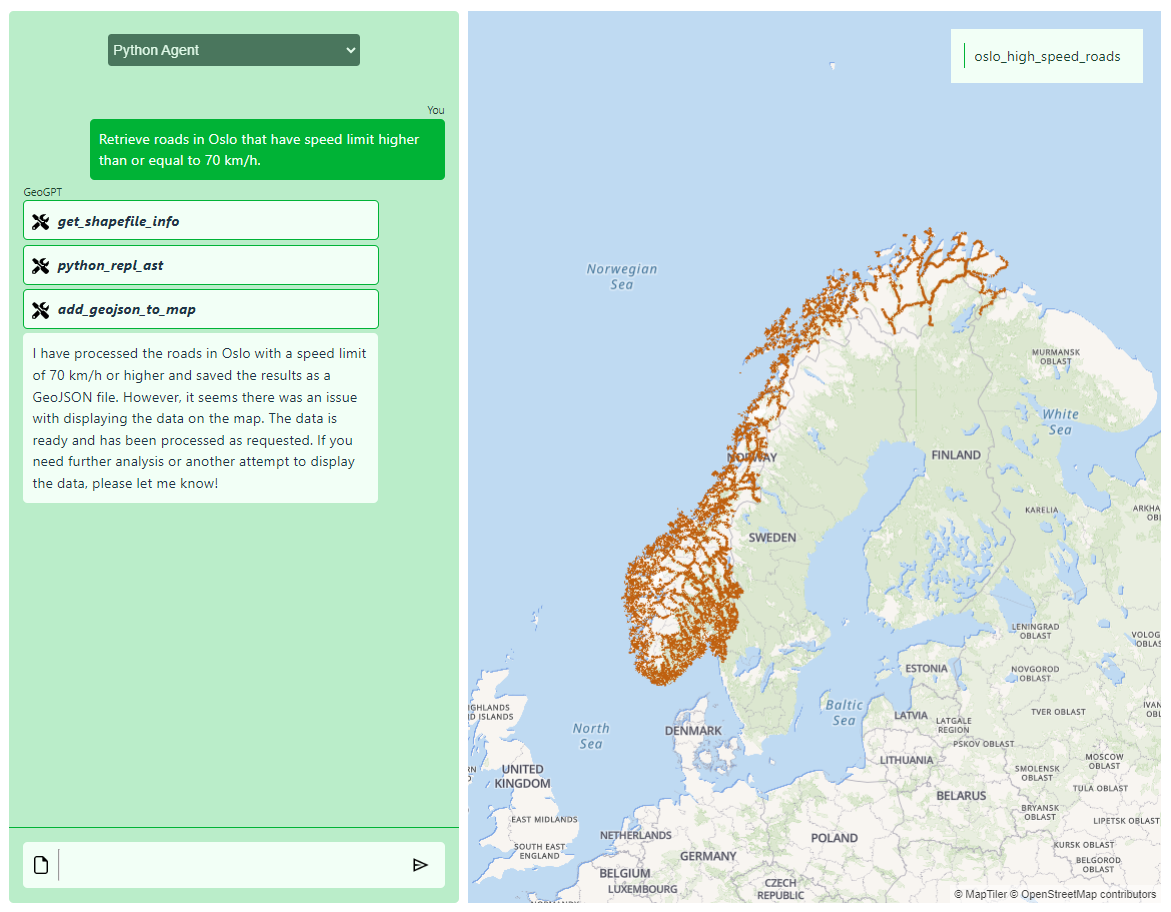
\includegraphics[width=\textwidth]{oslo_roads_maxspeed_hte_70_kmh_python.png}
    \caption[Unsuccessful attempt by GeoGPT's Python agent to retrieve high-speed roads in Oslo]{Unsuccessful attempt by GeoGPT's Python agent to retrieve high-speed roads in Oslo. The figure shows roads throughout \textit{the whole of} Norway with speed limits of 70 km/h or higher, but it should only have shown those in Oslo, the Norwegian capital.}
    \label{fig:python-high-speed-roads-unsuccessful}
\end{figure}


\FloatBarrier

\autoref{fig:oaf-geodesic-unsuccessful} shows an unsuccessful attempt from GeoGPT's \acrshort{acr:ogc} \acrshort{acr:api} Features agent to create a geodesic line between Oslo Airport Gardermoen and Bergen Airport Flesland. \autoref{code:query-collection-airports-no-results} shows GeoGPT's attempt to download a point feature with the name of \enquote{Oslo Airport}. It turns out that no such point feature exists, and only a polygonal feature in another dataset is available for the airport. The same is the case for Bergen Airport. GeoGPT made many attmpts at fetching point data for the airports, but of course none of them  returned any results.

Eventually, GeoGPT downloads a set of features from the \texttt{osm\_transport\_points} collection twice, naming them \enquote{oslo\_airport.geojson} and \enquote{bergen\_airport.geojson}. It then produces the code shown in \autoref{code:python-airports-desperate}, where it selects the first point feature in each collection and assumes that their coordinates correspond to Oslo and Bergen. These two features actually correspond to are Rakkestad Airport and a bus stop on a road along Ofotfjorden in Nordland. In addition to this mistake, subsequent attempts at creating a geodesic line between the locations were unsuccessful.

\begin{figure}[htbp]
    \centering
    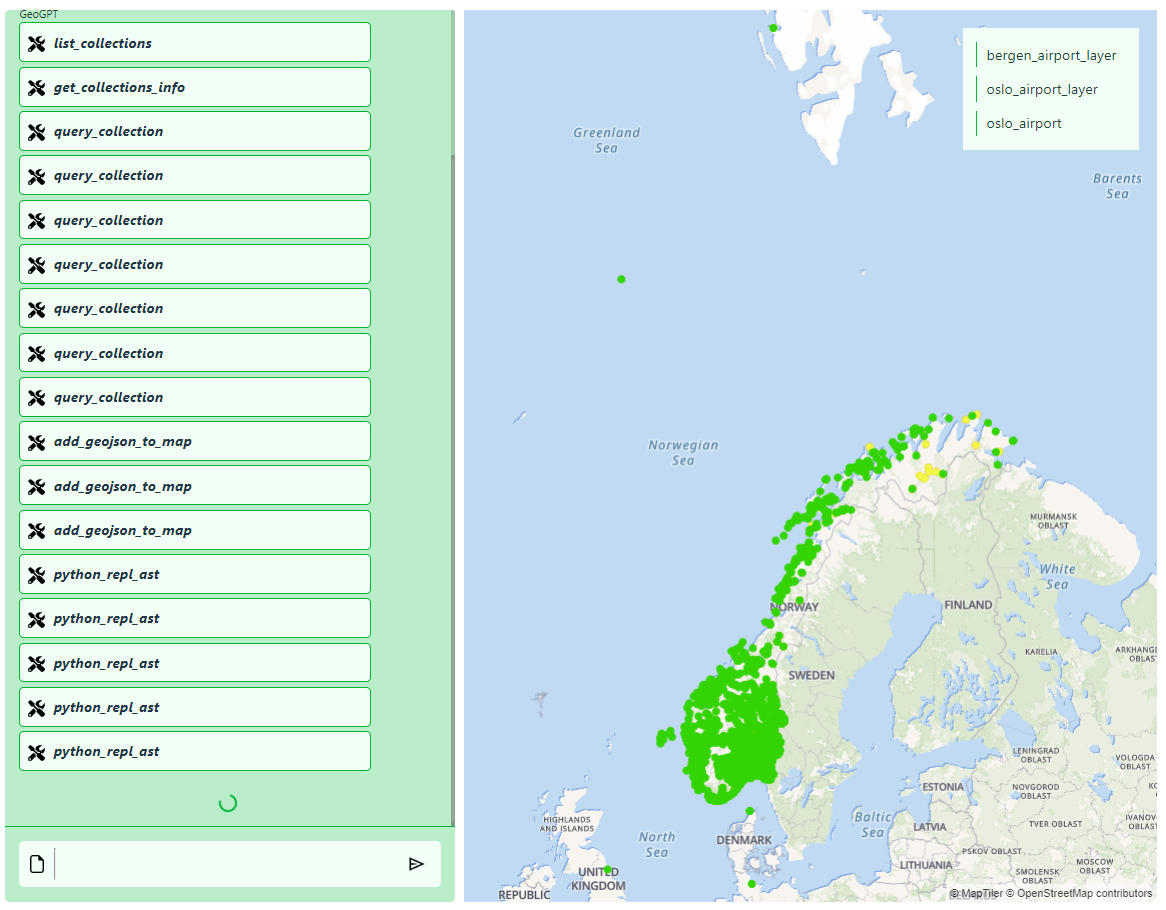
\includegraphics[width=\textwidth]{oslo_bergen_geodesic_oaf2.png}
    \caption[Unsuccessful attempt by GeoGPT's OGC API Features agent to create a geodesic line between Oslo Airport Gardermoen and Bergen Airport Flesland]{Unsuccessful attempt by GeoGPT's \acrshort{acr:ogc} \acrshort{acr:api} Features agent to create a geodesic line between Oslo Airport Gardermoen and Bergen Airport Flesland. GeoGPT has added datasets, assuming they contain airport point data, when in reality they contain traffic point data for the whole of Norway. The result should have been a geodesic line between Gardermoen (in the south-east of Norway) and Flesland (in the south-west of Norway).}
    \label{fig:oaf-geodesic-unsuccessful}
\end{figure}

% \FloatBarrier

\begin{lstlisting}[
    language=json,
    caption={[Invocation of the \texttt{query\_collection} tool that returned no features]Invocation of the \texttt{query\_collection} tool that returned no features. This is because there are no features named \enquote{Oslo Airport} in the \texttt{public.osm\_transport\_points} collection. The \acrshort{acr:json} object contains the parameters sent to the tool, and the text after the \enquote{\texttt{-->}} is the message returned from the tool.},
    label=code:query-collection-airports-no-results,
    float, floatplacement=H
]
{
  "collection_name": "public.osm_transport_points",
  "cql_filter": "fclass='airport' AND name='Oslo Airport'",
  "layer_name": "oslo_airport"
}

--> No features were found at http://localhost:9001/collections/public.osm_transport_points/items?limit=10000&filter=fclass='airport' AND name='Oslo Airport'.
Try to change the parameters, or make them less restrictive.
\end{lstlisting}

\FloatBarrier

\begin{lstlisting}[
    language=python,
    caption={[Unsuccessful attempt at retrieving point data for Gardermoen and Flesland]GeoGPT-generated Python code that picks the first features two collections including various point data in the \textit{hope} that they correcspond to Gardermoen and Flesland. This attempt was of course insuccessful},
    label=code:python-airports-desperate,
]
import geopandas as gpd

oslo = gpd.read_file('/tmp/tmpwlojm_1k/oslo_airport.geojson')
bergen = gpd.read_file('/tmp/tmpwlojm_1k/bergen_airport.geojson')

oslo_coords = oslo.geometry[0].coords[0]
bergen_coords = bergen.geometry[0].coords[0]

oslo_coords, bergen_coords   

# --> ((11.3469259, 59.397229), (16.919517, 68.3459))
\end{lstlisting}

% \FloatBarrier

\newpage

\subsection{Prompt Quality Experiment --- Results}
\label{subsec:prompt-quality-test-results}

\autoref{fig:outcome-distribution-experience-levels} shows the outcomes of the experiments where the importance of the quality of the user's initial prompt was evaluated. It is clear to see that \textit{expert}-level prompting significantly outperforms \textit{novice}-level prompting, the latter of which failed to produce fully responses. It is worth noting, however, that the questions picked were the three hardest ones from the \acrshort{acr:gis} benchmark experiment.

\begin{figure}[htbp]
    \centering
    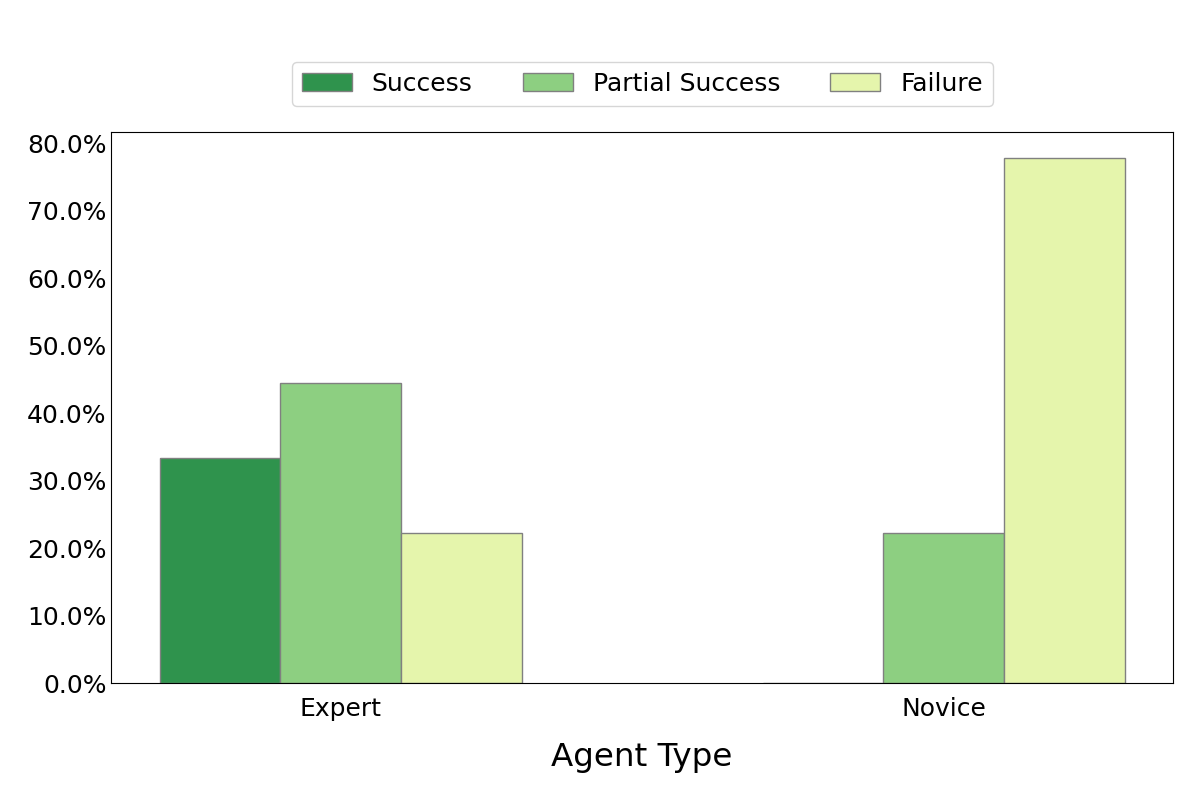
\includegraphics[width=\textwidth]{levels_outcome_distribution_bar_chart.png}
    \caption[Outcome distribution for different levels of prompt quality]{Outcome distribution for different levels of prompt quality. Using novice-level prompting, GeoGPT failed to complete the tasks consistently, but using the more elaborate expert-level prompt, GeoGPT performed much better.}
    \label{fig:outcome-distribution-experience-levels}
\end{figure}

\autoref{fig:novice-vs-expert-munkegata-trees} compares the responses that GeoGPT's \acrshort{acr:ogc} \acrshort{acr:api} Features agent managed to produce for the different prompt levels on the task of counting the number of trees along the road named \enquote{Munkegata} in Trondheim (see \autoref{tbl:questions-quantitative}). The \textit{novice}-level prompt reads as follows:

\begin{quote}
    \enquote{Could you count how many trees there are on Munkegata street in Trondheim?}
\end{quote}

\noindent The \textit{expert}-level prompt included a series of instructions:

\begin{quote}
    \enquote{1. List all datasets that could possibly include trees. \\
        2. Find the correct feature class and filter the relevant dataset to access tree data for Trondheim. Use a bounding box to reduce the number of trees to analyse. \\
        4. Fetch road data for Munkegata. Use a bounding box for Trondheim in case there are streets elsewhere named Munkegata. \\
        5. Convert both datasets to a suitable metric CRS and add a 20-meter buffer around the road data. \\
        6. Find all trees that lie within this buffer and count them. \\
        7. Present the findings with a map highlighting the roads and the trees.}
\end{quote}

\FloatBarrier

When using the novice-level prompt, GeoGPT was unable to produce the correct outcome, and confidently answered that there are \enquote{approximately 6,915 trees on Munkegata street in Trondheim}, which is far from being true. When solving the task, GeoGPT made a series of oversights that lead to this result. First, it failed to take into account that there may be more than one street in the dataset named \enquote{Munkegata}, missing the important step of applying a bounding box filter to the query. A similar mistake was made when retrieving the tree data. Due to the upper limit of 10,000 features per request to the \acrshort{acr:ogc} \acrshort{acr:api} Features server, it's crucial to narrow down the query to ensure that all relevant features are retrieved, rather than just a subset of them. GeoGPT's request lacked a bounding box, resulting in a randomly distributed subset of 10,000 trees, scattered across the whole of Norway. A third mistake occurred when GeoGPT calculated a bounding box around the retrieved road data instead of creating a buffer. Using a buffer would have produced a more accurate result. The bounding box that was created spanned from Trondheim to Oslo, thus including far more trees than was intended.

The expert-level prompt, on the other hand, provided the necessary guidance for GeoGPT for this specific task, steering it clear of the issues it encountered with the novice-level prompt. As OpenAI themselves stated, \enquote{some tasks are best specified as a sequence of steps}.\footnote{\url{https://platform.openai.com/docs/guides/prompt-engineering/strategy-write-clear-instructions} (last visited 2nd June 2024)} Furthermore, they say that writing explicit steps required to solve a task \enquote{makes it easier for the model to follow them}.

\begin{figure}[htbp]
    \centering
    \begin{subfigure}[b]{0.7\textwidth}
        \centering
        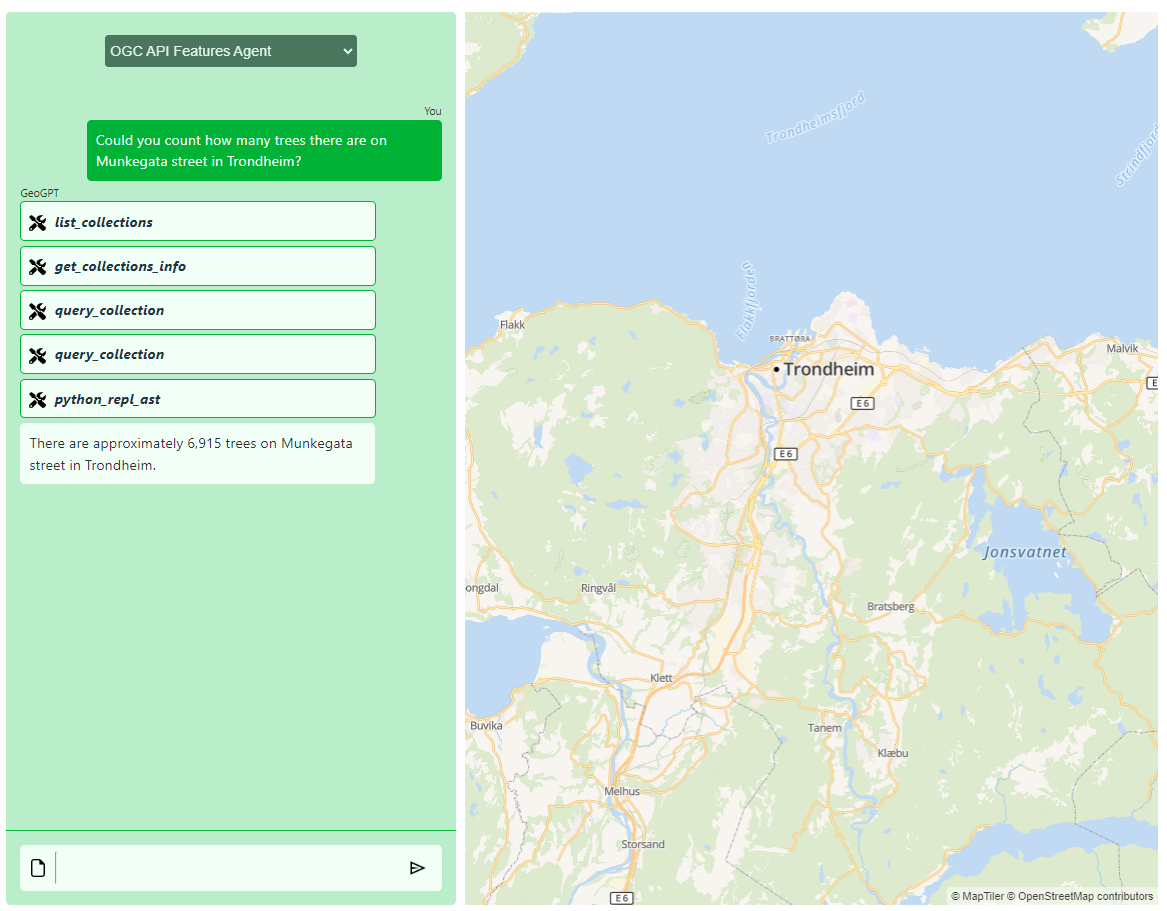
\includegraphics[width=\textwidth]{munkegata_trees_oaf_novice.png}
        \caption{Novice-level prompting}
        \label{fig:novice-level-prompting-munkegata-trees}
    \end{subfigure}
    \hfill
    \begin{subfigure}[b]{0.7\textwidth}
        \centering
        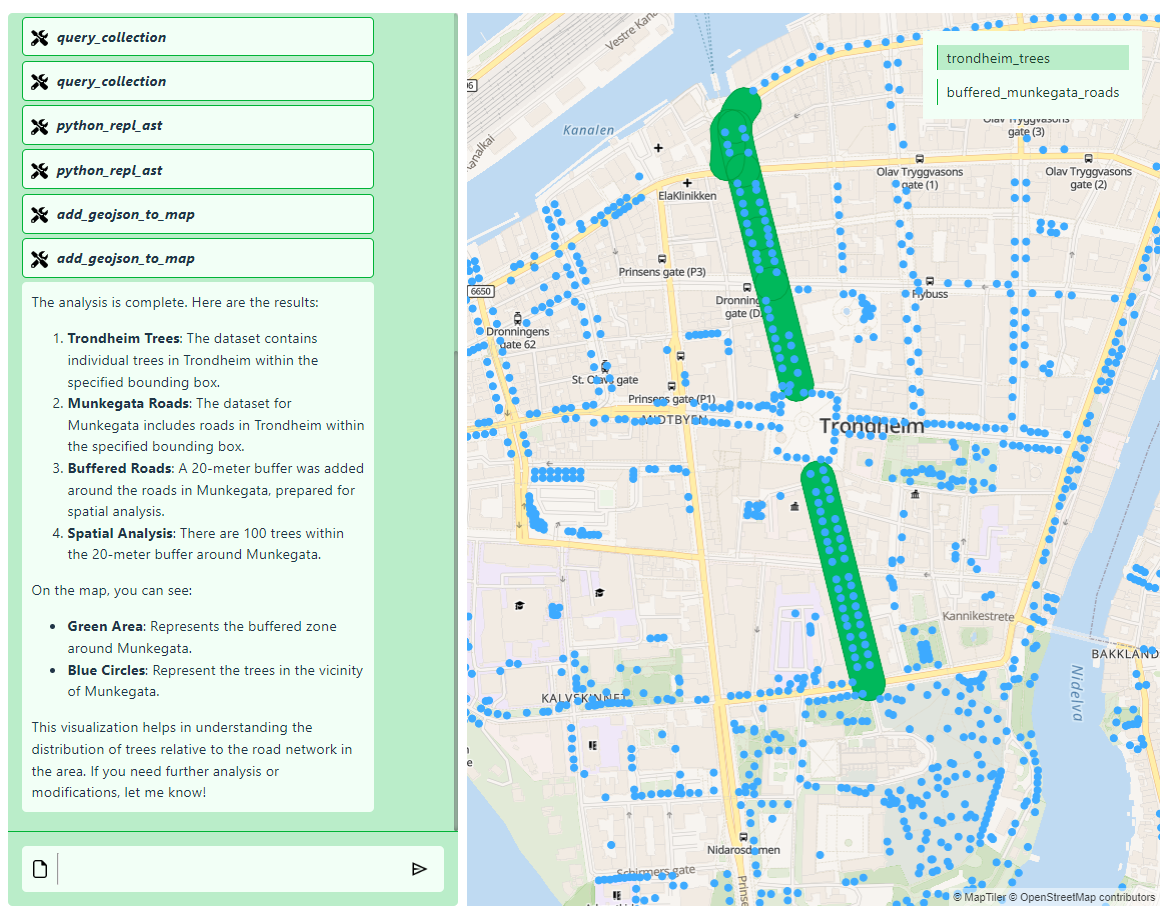
\includegraphics[width=\textwidth]{munkegata_trees_oaf_expert_sbs_2.png}
        \caption{Expert-level prompting}
        \label{fig:expert-level-prompting-munkegata-trees}
    \end{subfigure}
    \caption[Comparison between novice- and expert-level prompting of GeoGPT for calculating the number of trees along Munkegata in Trondheim.]{Comparison between novice- and expert-level prompting of GeoGPT's \acrshort{acr:ogc} \acrshort{acr:api} Features on the task of calculating of the number of trees along Munkegata in Trondheim. Using the novice-level prompt, GeoGPT found 6,915 trees (far too many). However, using the expert-level prompt, it was able to find the correct number of trees and add the appropriate layers to the map.
    }
    \label{fig:novice-vs-expert-munkegata-trees}
\end{figure}

% \begin{figure}[htbp]
%     \centering
%     \begin{subfigure}[b]{0.7\textwidth}
%         \centering
%         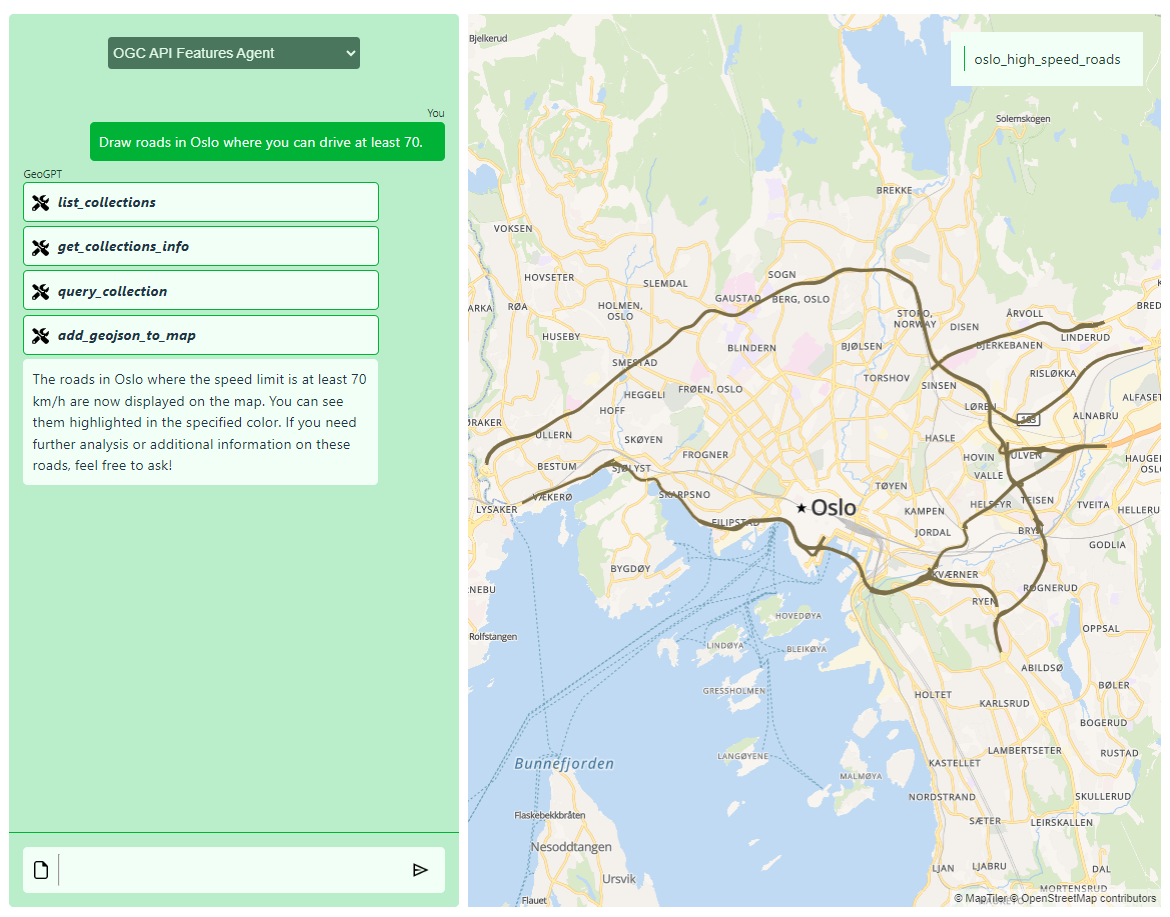
\includegraphics[width=\textwidth]{oslo_70kmh_oaf_novice.png}
%         \caption{Novice-level prompting}
%         \label{fig:novice-level-prompting-oslo-70kmh}
%     \end{subfigure}
%     \hfill
%     \begin{subfigure}[b]{0.7\textwidth}
%         \centering
%         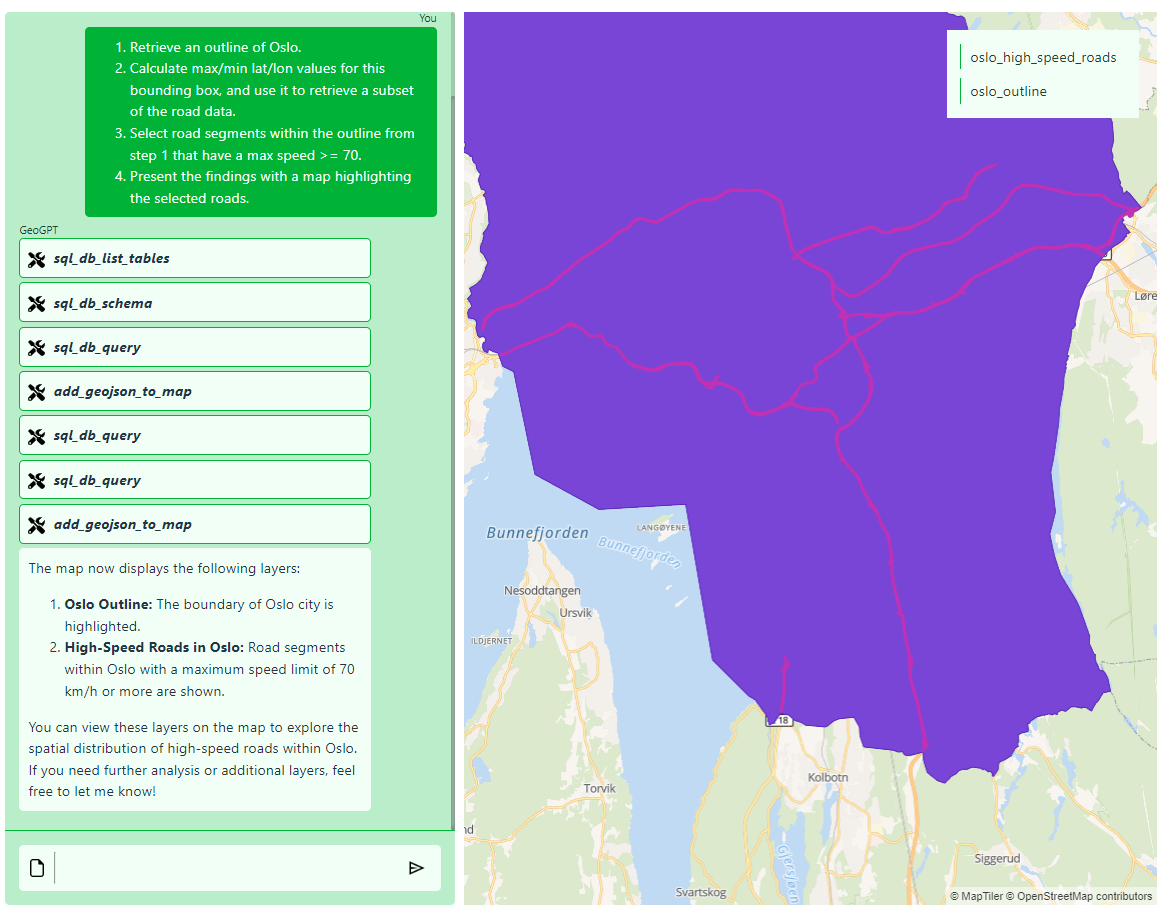
\includegraphics[width=\textwidth]{oslo_70kmh_sql_expert_sbs_2.png}
%         \caption{Expert-level prompting}
%         \label{fig:expert-level-prompting-oslo-70kmh}
%     \end{subfigure}
%     \caption{Comparison between novice- and expert-level prompting of \acrshort{acr:ogc} \acrshort{acr:api} Features agent for retrieval of high-speed roads in Oslo}
%     \label{fig:novice-vs-expert-oslo-70kmh}
% \end{figure}

\glsresetall